
\documentclass[12pt]{beamer}
\mode<presentation>{\usetheme{Madrid}} % Either Madrid or Rochester

\usefonttheme{professionalfonts}
\usenavigationsymbolstemplate{}

\usepackage[utf8]{inputenc}
%\usepackage[T1]{fontenc}
\usepackage{palatino}
%\usepackage{euler}
%\usepackage{amsmath}
%\usepackage{amsthm}
%\usepackage{amssymb}
%\usepackage{amsthm,geometry}  
%\usepackage[colorlinks=true]{hyperref}

\newtheorem{cor}{Corollary}
\newtheorem{lem}{Lemma}
\newtheorem{thm}{Theorem}
\newtheorem{defin}{Definition}
\newtheorem{proposition}{Proposition}

%polices
\newcommand{\msf}{\mathsf}
\newcommand{\mrm}{\mathrm}
\newcommand{\mbf}{\mathbf}
\newcommand{\mbb}{\mathbb}
\newcommand{\mcal}{\mathcal}
%polices

\newcommand{\bra}[1]{\langle #1|}
\newcommand{\ket}[1]{|#1 \rangle}
\newcommand{\braket}[2]{\langle #1|#2\rangle}
\newcommand{\ketbra}[1]{\ket{#1}\bra{#1}}
\newcommand{\ketb}[2]{\ket{#1}\bra{#2}}
\newcommand{\ident}{\mathbb{I}}
\DeclareMathOperator{\tr}{\mathrm{Tr}}
\DeclareMathOperator{\rank}{rank}
\DeclareMathOperator{\polylog}{polylog}
\newcommand{\mdag}{^{\dag}} % dag operator
\newcommand{\demi}{\frac{1}{2}}

\newcommand{\state}{{\rho^{AE}}}
\newcommand{\mixed}{\frac{\mathbb{I}}{d_{A}} \otimes \rho^E}
\newcommand{\tra}{\tr_A}
\newcommand{\cypher}{\mathcal{E}}

\newcommand{\mpr}{{\mrm{Pr}}}
\newcommand{\mtr}[1]{\mathrm{Tr}\left(#1\right)}%trace
\newcommand{\mtra}[1]{\mathrm{Tr}_{A}\left(#1\right)}%trace
\newcommand{\mtrb}[1]{\mathrm{Tr}_{B}\left(#1\right)}%trace
\newcommand{\p}{^{\prime}}


%Nombres
\newcommand{\mbR}{\mathbb{R}}
\newcommand{\mbZ}{\mathbb{Z}}
\newcommand{\mbQ}{\mathbb{Q}}
\newcommand{\mbC}{\mathbb{C}}
\newcommand{\mbN}{\mathbb{N}}
\newcommand{\mbI}{\mathbb{I}}
\newcommand{\mE}[1]{\mcal{E}(#1)}
\newcommand{\mO}[1]{\mcal{O}(#1)}
\newcommand{\mbE}{\mathbb{E}}
%Nombres

%notation de circuit
\newcommand{\mh}{\mathrm{H}}
\newcommand{\mx}{\mathrm{X}}
\newcommand{\my}{\mathrm{Y}}
\newcommand{\mzz}{\mathrm{Z}}
\newcommand{\ms}{\mathrm{S}}
\newcommand{\mt}{\mathrm{T}}
\newcommand{\mamp}{\frac{1}{\sqrt{2}}}
\newcommand{\cnot}{\mathrm{CNOT}}
\newcommand{\msx}{\sigma_{x}}
\newcommand{\msy}{\sigma_{y}}
\newcommand{\msz}{\sigma_{z}}

%Des choses essentielles ˆ la beautŽ d'un papier
\setlength{\parindent}{0cm}
\setlength{\parskip}{2ex plus 0.5ex minus 0.5ex}

% Pour cette présentation
\newcommand{\aeq}{\approx_{(a)}}
\newcommand{\wtA}{\widetilde{A}}
\newcommand{\wtB}{\widetilde{B}}
\newcommand{\whA}{\widehat{A}}
\newcommand{\whB}{\widehat{B}}
\DeclareMathOperator{\Typ}{typ}

\title{The decoupling approach to quantum information theory}

\author[Frédéric Dupuis]{Frédéric Dupuis\\
Université de Montréal\\
\strut\\
PhD Defense}
\date{Dec 21, 2009}

\begin{document}

\begin{frame}
\titlepage
\end{frame}

%\begin{frame}
%	\frametitle{Outline}
%	\tableofcontent
%\end{frame}
%----------------------------------------------------------

\begin{frame}
	\frametitle{Introduction}
	What is information theory?
	\begin{itemize}
		\item The study of information processing tasks:
		\begin{itemize}
			\item Data compression
			\item Data transmission through a noisy channel
		\end{itemize}
	\end{itemize}
	\emph{Quantum} information theory? Accomplishing these tasks with \emph{quantum} data or using quantum resources.
\end{frame}

\begin{frame}
	\frametitle{Introduction}
	So what's in this thesis? A general method to solve quantum information theory problems based on removing correlations between quantum systems. More specifically:
	\begin{itemize}
		\item A theorem that says how to remove correlations (``decouple'')
		\item How it can be used to recover many important QIT theorems
		\item New coding theorems for quantum channels with side information at the transmitter and broadcast channels
		\item A way to lock classical correlations in quantum states
	\end{itemize}
\end{frame}

\begin{frame}
	\frametitle{Outline}
	\begin{itemize}
		\item Introduction to channels and quantum information
		\item Coding by destroying correlations
		\item The decoupling theorem
		\item Channels with side information at the transmitter
		\item Locking classical correlations in quantum states
	\end{itemize}
\end{frame}

\begin{frame}
\frametitle{What is a channel?}
By ``channel'', I mean any physical means by which digital data can be communicated:
\begin{columns}
  \begin{column}{5cm}
    \begin{itemize}
	\item Radio link
        \item Fibre optics
	\item Telephone wire
	\item Etc\ldots
    \end{itemize}
  \end{column}
  \begin{column}{5cm}
    \begin{figure}
      \scalebox{0.20}{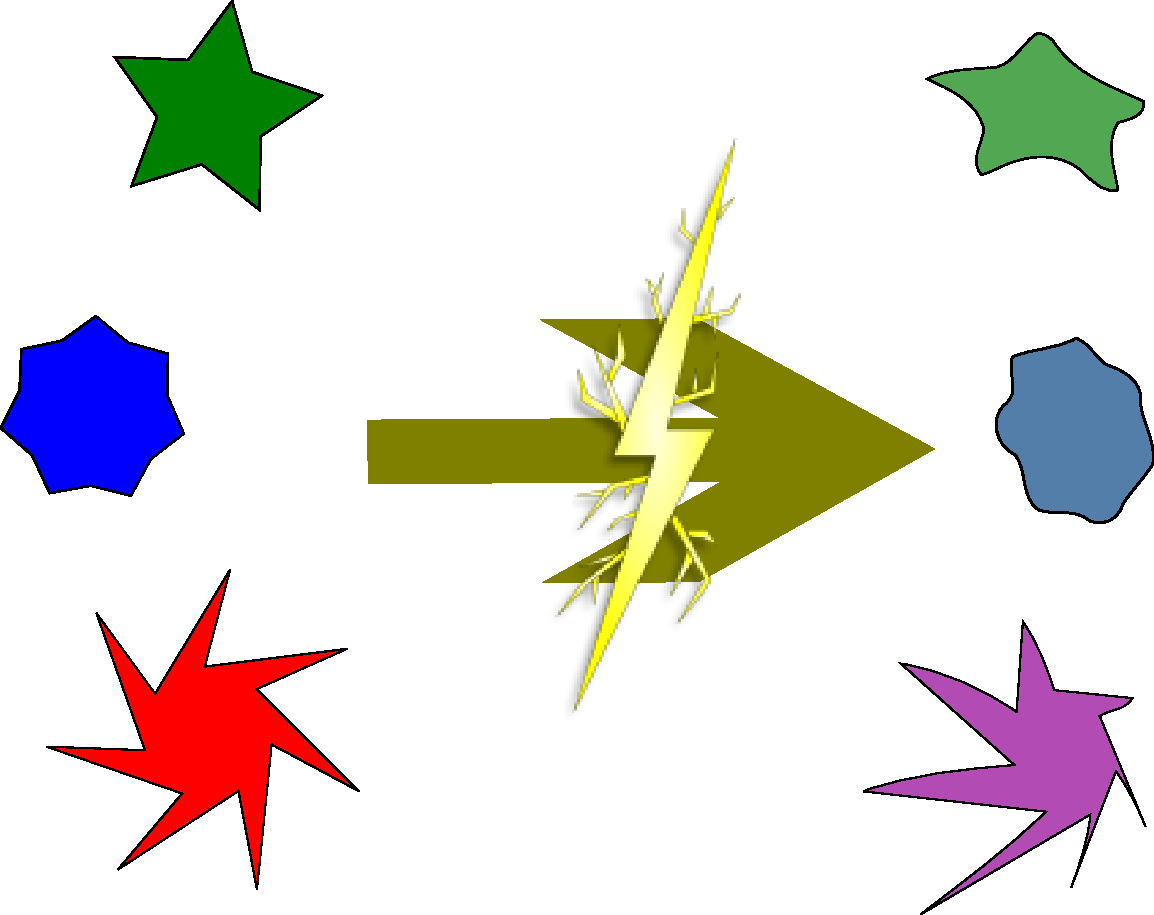
\includegraphics{canal-formes.pdf}}
    \end{figure}
  \end{column}
\end{columns}

Why can they transmit data?
\begin{itemize}
\item Choose an input
\item Send it into the channel, which corrupts it
\item Try to decipher which input was sent
\end{itemize}
\end{frame}

\begin{frame}
\frametitle{What is a channel?}
How do we model this mathematically?
\begin{itemize}
\item Input set $\mathcal{X}$
\item Output set $\mathcal{Y}$
\item Transition probability $p(y|x)$, $x \in \mathcal{X}, y \in \mathcal{Y}$
\end{itemize}

\begin{columns}
  \begin{column}{3cm}
    \begin{figure}
      \scalebox{0.20}{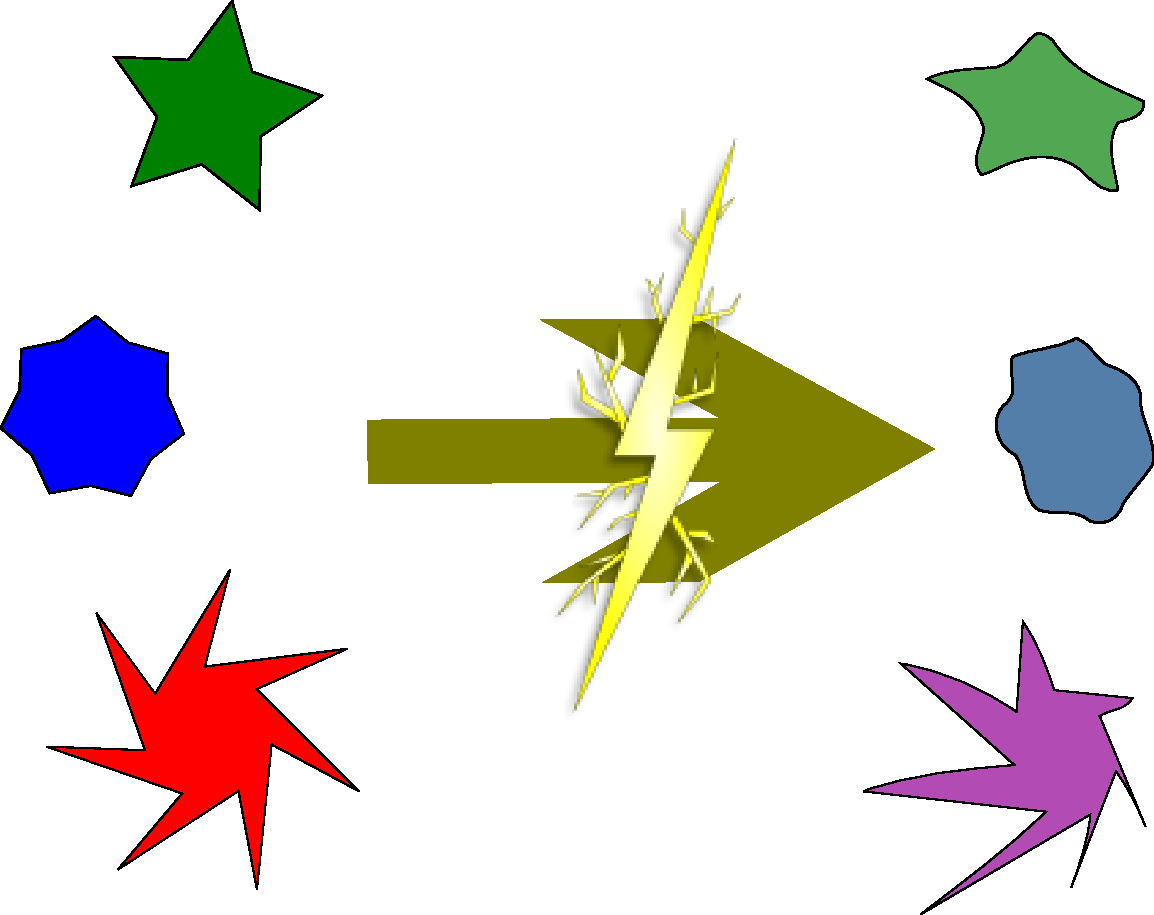
\includegraphics{canal-formes.pdf}}
    \end{figure}
  \end{column}
  \begin{column}{5cm}
    \begin{figure}
    \scalebox{1.00}{\input{canal-math.pdf_t}}
    \end{figure}
  \end{column}
\end{columns}
\end{frame}

\begin{frame}
\frametitle{Transmitting data through a channel}
Why use a channel? To send data:
\begin{itemize}
\item The message $m$ is a number from $1$ to $N$.
\item The encoder $E:\{0,\ldots,N\} \rightarrow \mathcal{X}$ associates each message to an input symbol from $\mathcal{X}$.
\item The decoder $D:\mathcal{Y} \rightarrow \{0,\ldots,N\}$ associates each output symbol from $\mathcal{Y}$ with a message estimate.
\end{itemize}
    \begin{figure}
    \hspace{-2.3cm}\scalebox{0.8}{\input{canal-enc-dec.pdf_t}}
    \end{figure}
\end{frame}

\begin{frame}
\frametitle{Transmitting data through a channel}
    \begin{figure}
    \hspace{-2.3cm}\scalebox{0.8}{\input{canal-enc-dec.pdf_t}}
    \end{figure}
Goals:
\begin{itemize}
\item $N$ as high as possible
\item $\Pr\{ m \neq \hat{m} \}$ as low as possible
\end{itemize}
The tradeoff between the two depends on the channel.
\end{frame}

\begin{frame}
\frametitle{Memoryless channels}
An interesting case: memoryless channels
    \begin{figure}
    \hspace{-2.3cm}\scalebox{0.8}{\input{canal-iid-enc-dec.pdf_t}}
    \end{figure}
This corresponds to using the same channel $n$ times; a very common occurrence!
\end{frame}

\begin{frame}
\frametitle{Memoryless channels}
    \begin{figure}
    \hspace{-2.3cm}\scalebox{0.8}{\input{canal-iid-enc-dec.pdf_t}}
    \end{figure}
In this case, it is possible to ensure that $\Pr\{ m \neq \hat{m} \} \rightarrow 0$ as $n \rightarrow \infty$ with fixed $(\log N)/ n$ [Shannon, 1949]
\end{frame}

\begin{frame}
\frametitle{Quantum channels}
	\begin{center}
		\Huge Quantum channels
	\end{center}
\end{frame}

\begin{frame}
\frametitle{Quantum information}
But first, a few words about quantum information\ldots
\begin{itemize}
\item Physical system that holds information:
\begin{itemize}
\item Classical: Sets $\mathcal{X}$, $\mathcal{Y}$,\ldots Size: log of number of elements in set
\item Quantum: Vector spaces $A$, $B$,\ldots Size: log of dimension of vector space
\end{itemize}
\item Possible value of information:
\begin{itemize}
\item Classical: An element $x$ of the set $\mathcal{X}$
\item Quantum: Pure state $\ket{\psi}^A$ in $A$
\end{itemize}
\item Probabilistic information:
\begin{itemize}
\item Classical: Probability distribution $p(x)$ over $\mathcal{X}$
\item Quantum: (Mixed) state $\rho^A$: matrix over $A$.
\end{itemize}
\end{itemize}
\end{frame}

\begin{frame}
\frametitle{Quantum information}
\begin{itemize}
\item Information-preserving transformations:
\begin{itemize}
	\item Classical: For each element in $\mathcal{X}$, pick a unique element in $\mathcal{Y}$.
\item Quantum: ``Partial isometries'' $V^{A \rightarrow B}$
\end{itemize}
\item General transformations:
\begin{itemize}
\item Classical: Channels $p(y|x)$
\item Quantum: ``CPTP maps'' $\mathcal{N}^{A \rightarrow B}$
\end{itemize}
\end{itemize}
\end{frame}

\begin{frame}
	\frametitle{Measuring information}
	How do we measure the amount of information? Entropies:
	\begin{itemize}
		\item Isolated state $\rho^{AB}$: $H_2(A|B)_{\rho}$. Uncertainty about $A$ when we have $B$. ``2-entropy''
		\item Multiple copies of state $\rho^{AB}$: $H(A|B)_{\rho}$. ``Shannon entropy''
	\end{itemize}
\end{frame}

\begin{frame}
\frametitle{Purifications}
\begin{itemize}
\item Given a mixed state $\rho^A$, there exists pure states $\ket{\psi}^{AB}$ such that $\rho^A = \psi^A$. We call $\ket{\psi}^{AB}$ a \emph{purification} of $\rho^A$.
\item Any two purifications $\ket{\psi}^{AB}$ and $\ket{\varphi}^{AC}$ of $\rho^A$ are related by a partial isometry $V^{B \rightarrow C}$:
\[ \ket{\varphi}^{AC} = V^{B \rightarrow C} \ket{\psi}^{AB} \]
\end{itemize}
\end{frame}

\begin{frame}
\frametitle{Quantum channels}
What are quantum channels concretely?

    \begin{itemize}
        \item Fibre optics
\item Optical link between Earth and satellites
	\item Quantum memory
	\item Etc\ldots
    \end{itemize}
\end{frame}

\begin{frame}
\frametitle{Sending quantum messages}
Why use a quantum channel $\mathcal{N}^{A' \rightarrow C}$? To send quantum data:
\begin{itemize}
\item The message is initially held in quantum system $M$.
\item The encoder $\mathcal{E}^{M \rightarrow A'}$ encodes the message into the input to the channel $A'$.
\item The decoder $\mathcal{D}^{C \rightarrow M}$ tries to recover the message from the channel output system $C$.
\end{itemize}
    \begin{figure}
    \scalebox{1}{\input{qcanal-enc-dec.pdf_t}}
    \end{figure}
\end{frame}

\begin{frame}
\frametitle{Sending quantum messages}
    \begin{figure}
    \scalebox{1}{\input{qcanal-enc-dec.pdf_t}}
    \end{figure}
How to measure the error probability? By comparing the above combination with
    \begin{figure}
    \scalebox{1}{\input{qcanal-ideal.pdf_t}}
    \end{figure}

We will want to show that
\[ \left\| \mathcal{D} \circ \mathcal{N} \circ \mathcal{E} - \mathcal{I} \right\|_{\diamond} \leqslant \varepsilon \]
\end{frame}

\begin{frame}
\frametitle{Sending quantum messages}
This is difficult to check directly: we would need to check every possible input state. Fortunately, we can only check $\Phi^{RM}$:
    \begin{figure}
    \scalebox{0.8}{\input{qcanal-enc-dec.pdf_t}}
    \end{figure}
\[ \left\| \mathcal{D} \circ \mathcal{N} \circ \mathcal{E} - \mathcal{I} \right\|_{\diamond} \leqslant \varepsilon \]
is (essentially) equivalent to  \vspace{-0.5cm}
    \begin{figure}
    \scalebox{0.8}{\input{qcanal-enc-dec-phi.pdf_t}}
    \end{figure}
\vspace{-0.5cm}
\[ \left\| (\mathcal{D} \circ \mathcal{N} \circ \mathcal{E})(\Phi^{RM}) - \Phi^{RM} \right\|_1 \leqslant \varepsilon \]
\end{frame}


\begin{frame}
\frametitle{Decoupling}
	\begin{center}
		\Huge Decoupling
	\end{center}
\end{frame}

\begin{frame}
\frametitle{Decoupling}
We can also purify CPTP maps: $\mathcal{N}^{A \rightarrow B}$ is equivalent to performing a partial isometry $U^{A \rightarrow BE}$, and then ignoring part of the output:
    \begin{figure}
    \scalebox{0.9}{\input{Nab.pdf_t}}
    \end{figure}
is equivalent to
    \begin{figure}
    \scalebox{0.9}{\input{UNab.pdf_t}}
    \end{figure}
\vspace{-0.5cm}We call $E$ the \emph{environment}.
\end{frame}

\begin{frame}
\frametitle{Decoupling}
    \begin{figure}
    \scalebox{0.8}{\input{qcanal-enc-dec-phi.pdf_t}}
    \end{figure}
becomes
    \begin{figure}
    \scalebox{0.8}{\input{qcanal-enc-dec-phi-pur.pdf_t}}
    \end{figure}
\end{frame}

\begin{frame}
\frametitle{Decoupling}
We then get
    \begin{figure}
    \scalebox{0.7}{\input{qcanal-enc-dec-phi-pur2.pdf_t}}
    \end{figure}
\begin{align*}
\ket{\psi}^{RM E_{\mathcal{D}} E_{\mathcal{N}} E_{\mathcal{E}}} &= \ket{\Phi}^{RM} \otimes \ket{\mbox{?}}^{E_{\mathcal{D}} E_{\mathcal{N}} E_{\mathcal{E}}}\\
\psi^{R E_{\mathcal{N}} E_{\mathcal{E}}} &= \pi^R \otimes \mbox{?}^{E_{\mathcal{N}} E_{\mathcal{E}}}
\end{align*}
\end{frame}

\begin{frame}
\frametitle{Decoupling}
    \begin{figure}
    \scalebox{0.8}{\input{qcanal-enc-dec-phi-pur3.pdf_t}}
    \end{figure}
\[ {\psi'}^{RE_{\mathcal{N}} E_{\mathcal{E}}} = \psi^{R E_{\mathcal{N}} E_{\mathcal{E}}} = \pi^R \otimes \mbox{?}^{E_{\mathcal{N}} E_{\mathcal{E}}} \]
\end{frame}

\begin{frame}
\frametitle{Decoupling}
    \begin{figure}
    \scalebox{0.8}{\input{qcanal-enc-dec-phi-pur3.pdf_t}}
    \end{figure}
Both $\ket{\psi}^{RME_{\mathcal{D}} E_{\mathcal{N}} E_{\mathcal{E}}}$ and $\ket{\psi'}^{RCE_{\mathcal{N}} E_{\mathcal{E}}}$ are purifications of $\pi^R \otimes \mbox{?}^{E_{\mathcal{N}} E_{\mathcal{E}}}$ $\Rightarrow$ they are related by a partial isometry $U_{\mathcal{D}}^{C \rightarrow M E_{\mathcal{D}}}$. 
\end{frame}

\begin{frame}
\frametitle{Decoupling}
    \begin{figure}
    \scalebox{0.8}{\input{qcanal-enc-dec-phi-pur3.pdf_t}}
    \end{figure}
To make sure a decoder exists, we only need to make sure that ${\psi'}^{RE_{\mathcal{N}} E_{\mathcal{E}}} \approx \pi^R \otimes \mbox{?}^{E_{\mathcal{N}} E_{\mathcal{E}}}$.
\end{frame}

\begin{frame}
\frametitle{Decoupling theorems}
\begin{itemize}
\item The same logic applies in many different information theory settings.
\item We need a way to ensure that two quantum systems are decoupled.
\item Two main methods used:
\begin{itemize}
\item Fully Quantum Slepian-Wolf (Abeyesinghe, Devetak, Hayden, Winter 2006)
\item State merging (Horodecki, Oppenheim, Winter 2005)
\end{itemize}
\item Common pattern: Apply random unitary, then do ``something''. Should be good on average.
\end{itemize}
\end{frame}

\begin{frame}
\frametitle{Fully Quantum Slepian-Wolf}
    \begin{figure}
    \scalebox{1.0}{\input{fqsw.pdf_t}}
    \end{figure}
    \[ \mbE_{U} \left\| \tr_{E}[U \cdot \psi^{AR}] - \pi^E \otimes \psi^R \right\|_1 \leqslant \sqrt{\frac{|E|}{|C|} 2^{-H_2(A|R)_{\psi}}} \]
\end{frame}

\begin{frame}
\frametitle{State merging}
\begin{figure}
    \begin{figure}
    \scalebox{1.0}{\input{merging.pdf_t}}
    \end{figure}
\[ \mbE_U \left\| \mathcal{M}^{A \rightarrow XL}(\psi^{AR}) - \pi^{XL} \otimes \psi^R \right\|_1 \leqslant \sqrt{|L| 2^{-H_2(A|R)_{\psi}}} \]
\end{figure}
\end{frame}

\begin{frame}
\frametitle{Decoupling theorem}
We can generalize these:
    \begin{figure}
    \scalebox{0.9}{\input{decoupling-thm.pdf_t}}
    \end{figure}
\[ \mbE_U \left\| \mathcal{T}^{A \rightarrow E}(\psi^{AR}) - \mathcal{T}(\pi^A) \otimes \psi^R \right\|_1 \leqslant \sqrt{2^{-H_2(A'|E)_{\omega} -H_2(A|R)_{\psi}}} \]
\end{frame}

\begin{frame}
\frametitle{Decoupling theorem}
\begin{itemize}
\item We recover FQSW and state merging (just use the $\mathcal{T}$ that corresponds to them)
\item Much more general and flexible
\end{itemize}
\end{frame}


\begin{frame}
\frametitle{Decoupling theorem}
An even more general version: there exists a $V^{A \rightarrow A'}$ such that
\vspace{-0.5cm}
    \begin{figure}
    \scalebox{0.9}{\input{decoupling-thm2.pdf_t}}
    \end{figure}
\vspace{-1cm}
\begin{multline*}
 \left\| \mathcal{T}^{A' \rightarrow E}(U \cdot \psi^{AR}) - \mathcal{T}(\pi^A) \otimes \psi^R \right\|_1\\
\lesssim \sqrt{2^{-H^{\varepsilon}_2(A''|E)_{\omega} -H^{\varepsilon}_2(A|R)_{\psi}}} + \sqrt{2^{H^{\varepsilon}_{\max}(A)_{\psi} - H_2^{\varepsilon}(A'')_{\omega}}} 
\end{multline*}
\end{frame}

\begin{frame}
	\frametitle{One-shot quantum channel coding}
	By purifying this, we get a channel coding theorem:
    \begin{figure}
    \scalebox{0.92}{\input{one-shot-channel-coding.pdf_t}}
    \end{figure}
    Similar to Buscemi and Datta (2009), but with quantum side-information at Bob.
\end{frame}

\begin{frame}
	\frametitle{Quantum channel coding}
	Special case of interest: $\mathcal{T} = \mathcal{N}^{\otimes n}$:
	\vspace{-1cm}
    \begin{figure}
    \scalebox{0.9}{\input{decoupling-thm2-iid.pdf_t}}
    \end{figure}
\end{frame}

\begin{frame}
	\frametitle{Quantum channel coding}
	Recall that:
\begin{multline*}
 \left\| \mathcal{T}^{A' \rightarrow E}(U \cdot \psi^{AR}) - \mathcal{T}(\pi^A) \otimes \psi^R \right\|_1\\
\lesssim \sqrt{2^{-H^{\varepsilon}_2(A''|E)_{\omega} -H^{\varepsilon}_2(A|R)_{\psi}}} + \sqrt{2^{H^{\varepsilon}_{\max}(A)_{\psi} - H_2^{\varepsilon}(A'')_{\omega}}} 
\end{multline*}
But when $\mathcal{T} = \mathcal{N}^{\otimes n}$, 
\begin{align*}
H_2^{\varepsilon}({A''}^n|E^n)_{\omega^{\otimes n}} &\rightarrow nH(A''|E)_{\omega}\\
H_2^{\varepsilon}({A''}^n)_{\omega^{\otimes n}} &\rightarrow nH(A'')_{\omega}
\end{align*}
[Tomamichel, Colbeck, Renner 2008]. Hence,
\begin{multline*}
	\left\| \mathcal{N}^{\otimes n}(U \cdot \psi^{AR}) - \mathcal{N}^{\otimes n}(\pi^A) \otimes \psi^R \right\|_1\\
\lesssim \sqrt{2^{-nH(A''|E)_{\omega} -H^{\varepsilon}_2(A|R)_{\psi}}} + \sqrt{2^{H^{\varepsilon}_{\max}(A)_{\psi} - nH(A'')_{\omega}}} 
\end{multline*}
\end{frame}

\begin{frame}
	\frametitle{Quantum channel coding}
    \begin{figure}
    \scalebox{0.9}{\input{iid-channel-coding.pdf_t}}
    \end{figure}
    \begin{align*}
	    \log|M| &< -H(A''|E)_{\omega}
    \end{align*}
    [Lloyd, Shor, Devetak] 
\end{frame}

\begin{frame}
	\frametitle{Channels with side information at the transmitter}
	\begin{center}
	\Huge Channels with side information at the transmitter
	\end{center}
\end{frame}

\begin{frame}
	\frametitle{Channels with side information at the transmitter}
	What is a (classical) channel with side information at the transmitter?
	\begin{itemize}
		\item $p_{Y|XS}(y|x,s)$
		\begin{itemize}
			\item Input $x \in \mathcal{X}$	
			\item Output $y \in \mathcal{Y}$	
			\item State $s \in \mathcal{S}$	
			\item Probability distribution over $S$ fixed by channel: $p_S(s)$	
		\end{itemize}
	\item $s$ is known to the transmitter ahead of time.	
	\end{itemize}
\end{frame}

\begin{frame}
	\frametitle{Channels with side information at the transmitter}
	Consider an $n$-bit memory device, where each bit can be in one of 3 states:
	\begin{itemize}
		\item Stuck at 0: No matter what we write, we get 0. Happens with probability $\varepsilon/2$.
		\item Stuck at 1. Happens with probability $\varepsilon/2$.
		\item Works perfectly. Happens with probability $1-\varepsilon$.
	\end{itemize}
	We can test the memory before writing to it, but not when reading from it.
\end{frame}

\begin{frame}
	\frametitle{Quantum channels with side information at the transmitter}
	A quantum version of this makes sense. For example, an $n$-qubit quantum memory device, with each qubit either
	\begin{itemize}
		\item Stuck at 0: No matter what we write, we get $\ket{0}$. Happens with probability $\varepsilon/2$.
		\item Stuck at 1. Happens with probability $\varepsilon/2$.
		\item Functioning perfectly. Happens with probability $1-\varepsilon$.
	\end{itemize}
	We can test the memory before writing to it, but not when reading from it.
\end{frame}

\begin{frame}
	\frametitle{Quantum channels with side information at the transmitter}
	General quantum case:
	\begin{itemize}
		\item Alice has a quantum system $S$ in her hands which is correlated with what the channel will do.
	\end{itemize}
    \begin{figure}
    \scalebox{0.9}{\input{side-info-explain.pdf_t}}
    \end{figure}
\end{frame}

\begin{frame}
	\frametitle{Coding theorem}
	We can use the decoupling theorem to get a coding theorem for these channels:
    \begin{figure}
    \scalebox{0.9}{\input{side-info-coding.pdf_t}}
    \end{figure}
\end{frame}

\begin{frame}
	\frametitle{Locking classical information in quantum states}
	\begin{center}
	\Huge Locking classical information in quantum states
	\end{center}
	Joint work with Patrick Hayden and Debbie Leung
\end{frame}

\begin{frame}
	\frametitle{Locking classical information in quantum states}
	\begin{itemize}
	\item We can encode $n$ classical bits into $n$ qubits.
	\item We can also ``lock'' $n$ classical bits into quantum states as follows:
	\begin{itemize}
	\item Perform a unitary on the message
	\item Split the message into a big part $C$ and a tiny ``key'' $K$
	\item Any measurement result on $C$ is uncorrelated with the message
	\end{itemize}
	\end{itemize}
\end{frame}

\begin{frame}
	\frametitle{Locking classical information in quantum states}
    \begin{figure}
    \scalebox{0.9}{\input{locking1.pdf_t}}
    \end{figure}
\end{frame}

\begin{frame}
	\frametitle{Locking classical information in quantum states}
    \begin{figure}
    \scalebox{0.9}{\input{locking2.pdf_t}}
    \end{figure}
\end{frame}

\begin{frame}
	\frametitle{Just like encryption?}
	Not surprised? Isn't that what we do when we encrypt a file? Not quite\ldots
	\begin{itemize}
	\item Message: A number from 1 to 10
	\item Key: a single bit
	\item Given a classical $C$, I can always narrow down the message to two possibilities out of 10. Hence, $C$ is very correlated with the message.
	\item To prevent correlations, the key must be as big as the message.
	\end{itemize}
	Quantumly: an $n$-bit message with a $\polylog(n)$ key is possible.
\end{frame}

\begin{frame}
	\frametitle{Proof sketch}
	\begin{itemize}
		\item For any fixed measurement, we can use the decoupling theorem to show that, when we select $U$ at random, on average the final state is decoupled.
	\item We can also show that this is true with very high probability, so the probability of bad decoupling for a given measurement is very low.
	\item So low that:
		\begin{multline*}
		 \left( \mbox{Prob of bad measurement}\right)\\
		 \times (\mbox{\# of possible measurements}) < 1
		\end{multline*}
	\item So there exists a $U$ that gives good decoupling for \emph{every} measurement.
	\item How to count possible measurements? Somewhat complicated\ldots
	\end{itemize}
\end{frame}

\begin{frame}
	\frametitle{Previous work on locking}
	Pick random $U$, key = choice of $U$:
	\begin{itemize}
		\item DiVincenzo, Horodecki, Leung, Smolin, Terhal 2004
		\item Hayden, Leung, Shor, Winter 2004
	\end{itemize}
	This work:
	\begin{itemize}
		\item Quantum key
		\item Success criterion: trace distance from decoupled state instead of accessible information
	\end{itemize}
\end{frame}

\begin{frame}
	\frametitle{Conclusion}
	\begin{itemize}
	\item Showed a general decoupling theorem
	\item Can be used in very diverse problems in quantum information theory and unifies them
	\item Showed coding theorems for channels with side information at the transmitter
	\item Showed (in the thesis!) coding theorems for broadcast channels
	\item Showed how to lock classical correlations into quantum states
	\end{itemize}
\end{frame}

\begin{frame}
	\frametitle{What about the future?}
	\begin{itemize}
	\item We have not used the decoupling theorem to its full potential yet
	\item Could be used to show protocols for channels with memory
	\item Other types of channels
	\item Optimality?
	\item Explicit protocols (with high concentration)
	\end{itemize}
\end{frame}

\begin{frame}
	\frametitle{The End}
	\begin{center}
		\Huge Thank you!
	\end{center}
\end{frame}

\end{document}
